%----------------------------------------------------------------------------------------
%	CHAPTER 3: Ripa Exchange
%----------------------------------------------------------------------------------------

\chapterimage{chapter_head_3_Singapore.jpg} % Chapter heading image

\chapter{The Ripa Exchange}
Ripa Exchange is an crypto asset (fiat money or cryptocurrency or something) marketplace, following the latest 
industry standards and resting in the principles of ``\textit{open source, secure and efficient}''. Ripa Exchange
aims to serve a platform for crypto-currency enthusiasts by providing a safe, secure, UI responsive, customizable 
and easy to use exchange that embraces open source principles and public trust.\\\\
Ripa Exchange is implemented with the Rails framework and other cutting-edge technology and will be migrated to an
hybrid-decentralized exchange where all exchanges in the Ripa network will share liquidity thanks to RLSP technology.

\section{Mission}
\begin{quotation}
	``\textit{Our mission is to build the world best open source crypto asset marketplace with a high performance trading engine 
	and safety which can be trusted and enjoyed by users. Additionally we want to move the crypto currency exchange technology 
	forward by providing support and add new features. We are helping people to build easy their own exchange around the world.}''
\end{quotation}

Help is greatly appreciated, feel free to submit pull-requests or open issues in our \href{https://github.com/RipaEx}{GitHub repositories}.

\section{Features}
A free, transparent and internationalized open source crypto currency exchange.

\tcbset{featureBox/.style={colback=yellow!10!white,colframe=white!20!black,
equal height group=nobefaf,width=(\linewidth-1pt)/3, height=5.0cm, nobeforeafter,
	center title,
	valign=top, halign=left}}
\begin{tcolorbox}[featureBox,
	title=\textsc{Open Source} \faCircleONotch]

	\small	All source code are fully released under the terms of the MIT License.\\\vspace{5mm}
	\tiny Ripa Exchange is a customizable cryptocurrency exchange solution architecture enables easy connection to KYC/AML, 
	authentication, ETL/reporting, and other services.
\end{tcolorbox}
\begin{tcolorbox}[featureBox,
	title=\textsc{Compliant} \faCheck]

	\small	International KYC/AML standards.\\\vspace{5mm}
	\tiny Ripa Exchange KYC efficiently submits and exchanges KYC information 
	to meet the banking supervisory standards and comply with Customer Due Diligence (CDD) requirements.
\end{tcolorbox}
\begin{tcolorbox}[featureBox,
	title=\textsc{Transparent \& Configurable} \faCogs]

	\small	Customize in your own way\\\vspace{5mm}
	\tiny Major functions have been embedded in the source code – neat registration and log-in interface, 
	personalized deposit and withdraw procedure, best match of bid and ask, etc. These functions are comprehensive 
	and are ready to use with no extra work needed. 
\end{tcolorbox}

\begin{tcolorbox}[featureBox,
	title=\textsc{Internationalization} \faLanguage]

	\small	All users are able to view Ripa Exchange in a language to their best convenience.\\\vspace{5mm}
	\tiny Supporting many common languages, Ripa Exchange makes it easy for users to operate in their mother tongue. 
	You are encouraged to contribute to our language variety. Users will benefit from your efforts.
\end{tcolorbox}
\begin{tcolorbox}[featureBox,
	title=\textsc{Proof of Solvency} \faUsers]

	\small	Easy deployable PoS.\\\vspace{5mm}
	\tiny Ripa Exchange Proof of Solvency (PoS) allows users to verify 
	the solvency of the Ripa Exchange based cryptocurrency exchange without compromising user privacy.
\end{tcolorbox}
\begin{tcolorbox}[featureBox,
	title=\textsc{Multi-Accounts Trading} \faHandSpockO]

	\small	Easy currency configuration.\\\vspace{5mm}
	\tiny Ripa Exchange allows to create multiple accounts and trading in multiple currencies. 
	Ripa Exchange makes it is easy to trade different currencies.
\end{tcolorbox}

\begin{tcolorbox}[featureBox,
	title=\textsc{Multi-Accounts Users} \faSuitcase]

	\small	Easy account configuration.\\\vspace{5mm}
	\tiny Ripa Exchange allows to create multiple login accounts Google, Facebook, Twitter and FIDO Alliance
	login standards to secure your account.
\end{tcolorbox}
\begin{tcolorbox}[featureBox,
	title=\textsc{Enterprise Exchange} \faInstitution]

	\small	Start small, grow big.\\\vspace{5mm}
	\tiny Ripa Exchange enterprise exchange features include a high-performance matching engine, 
	scalable distributed worker threads, and SMS 2-factor authentication.
\end{tcolorbox}
\begin{tcolorbox}[featureBox,
	title=\textsc{Functional \& Intuitive} \faIntersex]

	\small	For the new trader, for the experienced trader.\\\vspace{5mm}
	\tiny Clean, user friendly registration and login interface. 
	Personalized deposit and withdraw procedure and a built-in proof-of-solvency audit.
\end{tcolorbox}

\section{Functional Analysis}
\todo{TODO: more details here}
\begin{enumerate}
	\item \textsc{Why Redis-RabbitMQ is needed}:
	\item \textsc{Why NodeJS}: 
	\item \textsc{Why Pusher}:
	\item \textsc{ER MySQL}:
	\item \textsc{Ruby folders hierarchy}:
\end{enumerate}

\section{Technology Stack}
\todo{TODO: more details here}
\begin{itemize}
	\item \textbf{\textsc{Ruby on Rails}}:
	\item \textbf{\textsc{MySQL}}: 
	\item \textbf{\textsc{Redis}}:
	\item \textbf{\textsc{RabbitMQ}}:
	\item \textbf{\textsc{NodeJS}}:
	\item \textbf{\textsc{Pusher}}:
\end{itemize}

\section{User Interface}
Ripa Exchange user interface is based on Peatio user interface a UI responsive user interface built in Ruby on Rails and 
completely separated from the exchange order engine.
Design for a customised UI are in place to offer to Ripa Exchange users the best experience on all devices: here you can find
some screenshots of the current exchange interface design.

\subsection{End-User Interface}
Following some screenshot of the end-user Ripa Exchange-Peatio interface: 
\textcolor{darkred}{those screenshots are a work in progress and they may not represents the user interface of the final product}
\begin{center}
	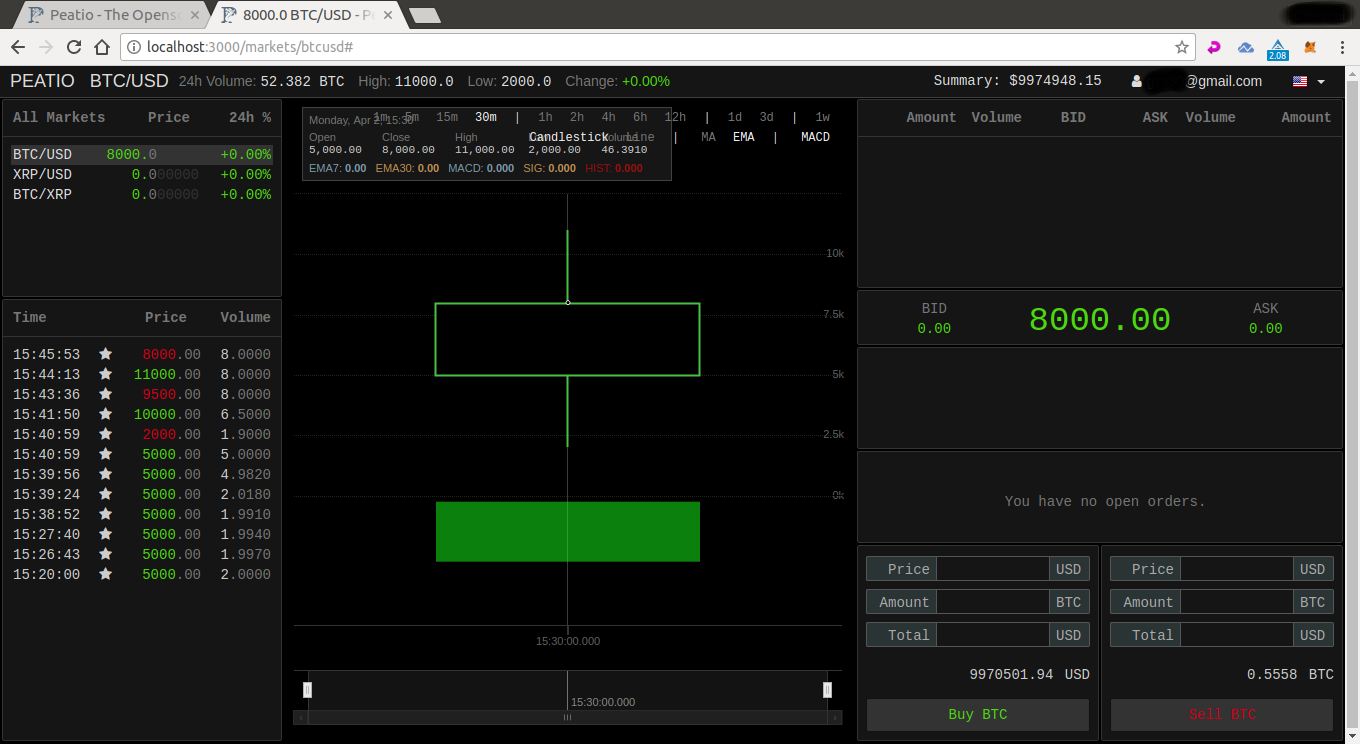
\includegraphics[width=\textwidth*2/3,height=\textheight,keepaspectratio]{RE_TradingUIC}
	\captionof{figure}{Ripa Exchange trading UI}
	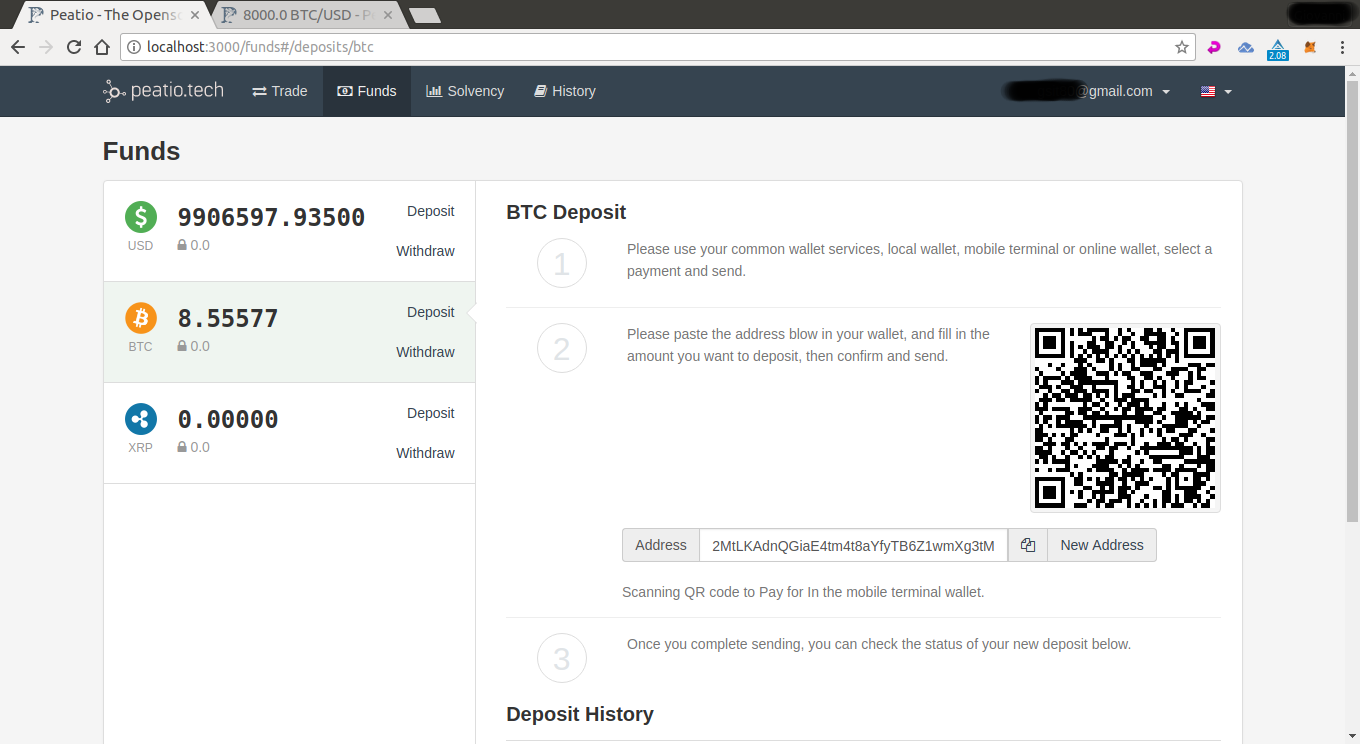
\includegraphics[width=\textwidth*2/3,height=\textheight,keepaspectratio]{RE_depositBTCC}
	\captionof{figure}{Ripa Exchange deposit/whitdraw}
	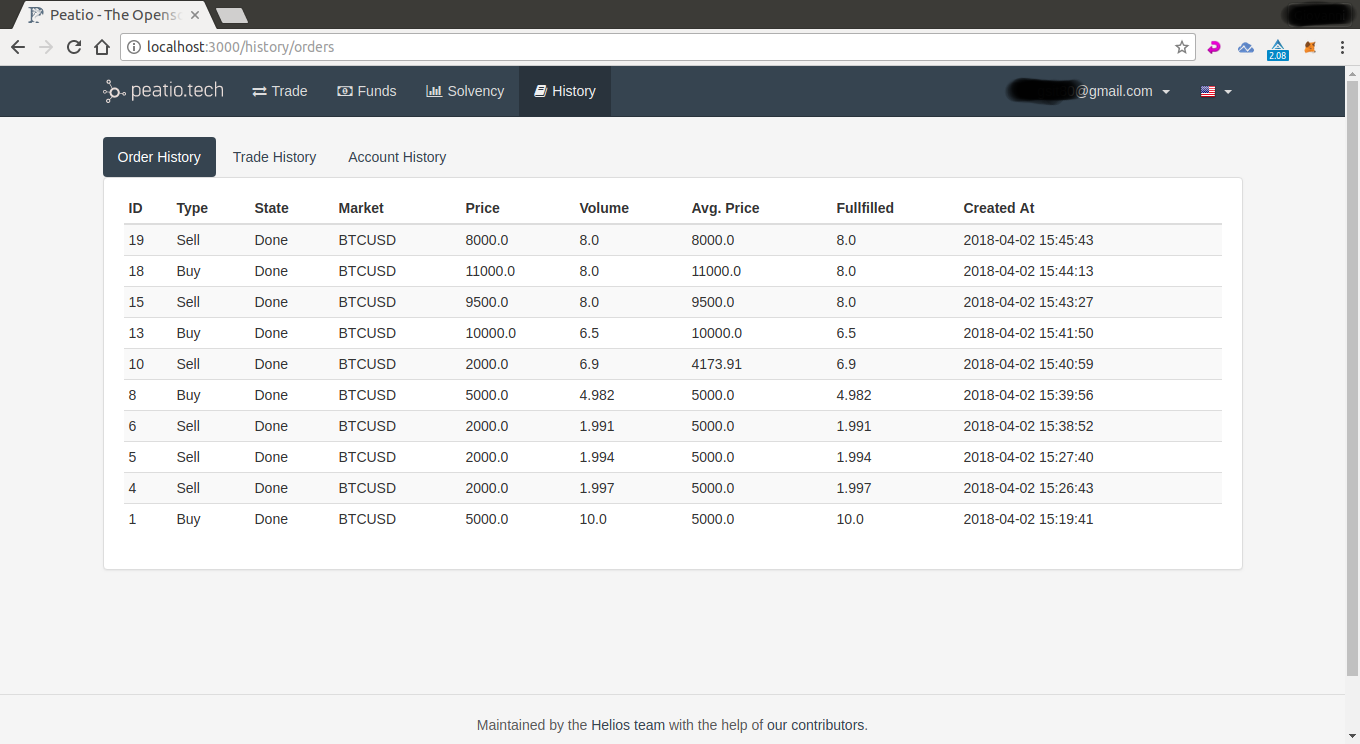
\includegraphics[width=\textwidth*2/3,height=\textheight,keepaspectratio]{RE_historyC}
	\captionof{figure}{Ripa Exchange order history}
	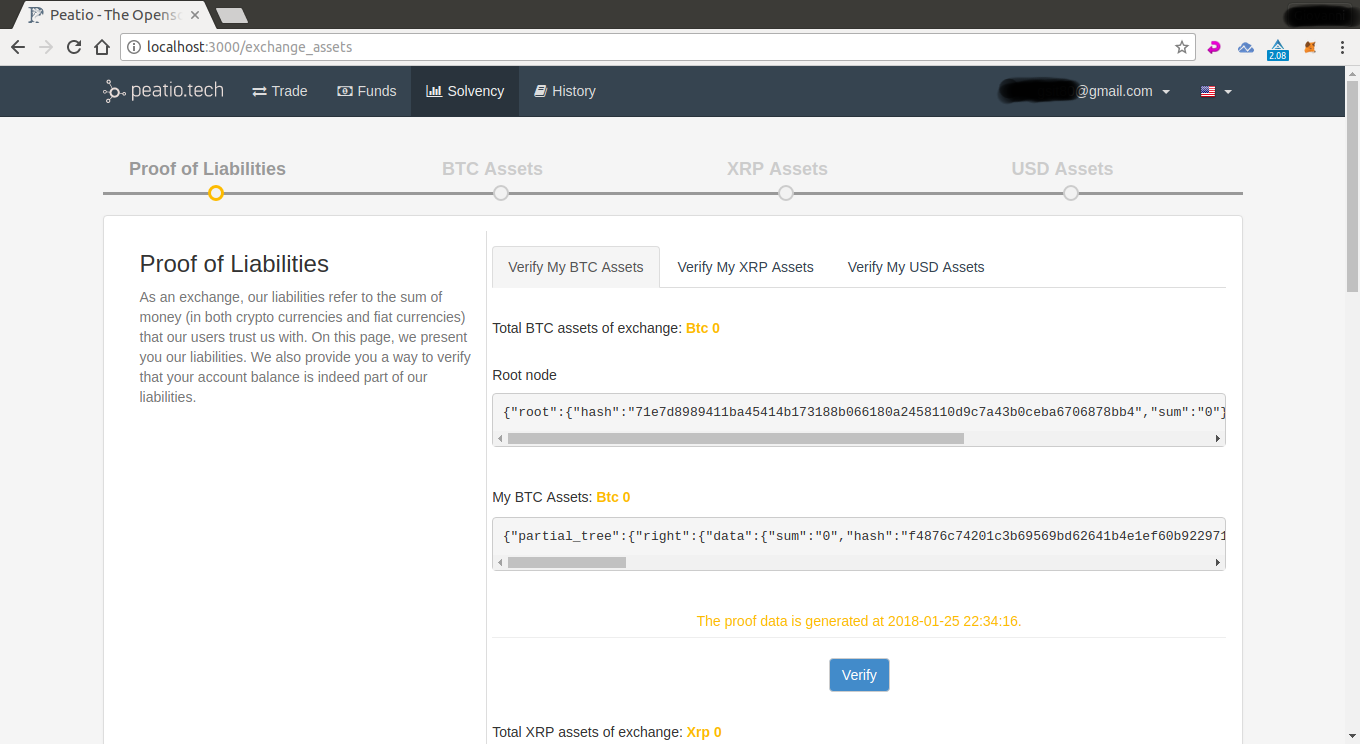
\includegraphics[width=\textwidth*2/3,height=\textheight,keepaspectratio]{RE_solvencyC}
	\captionof{figure}{Ripa Exchange solvency screen}
\end{center}

\subsection{Admin Interface}
Following some screenshot of the administrative console of Ripa Exchange-Peatio interface: 
\textcolor{darkred}{those screenshots are a work in progress and they may not rapresents the user interface of the final product}
\begin{center}
	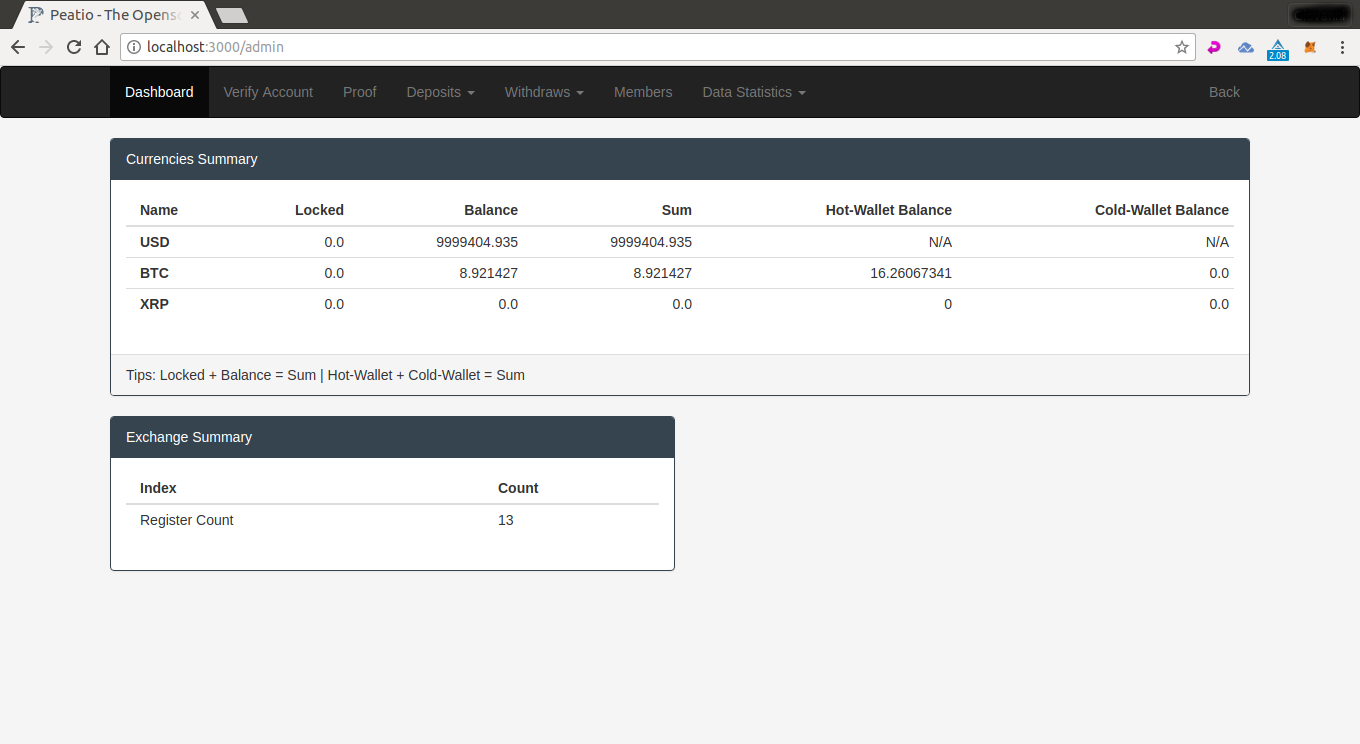
\includegraphics[width=\textwidth*2/3,height=\textheight,keepaspectratio]{RE_adminDashboardC}
	\captionof{figure}{Ripa Exchange Admin console dashboard}
	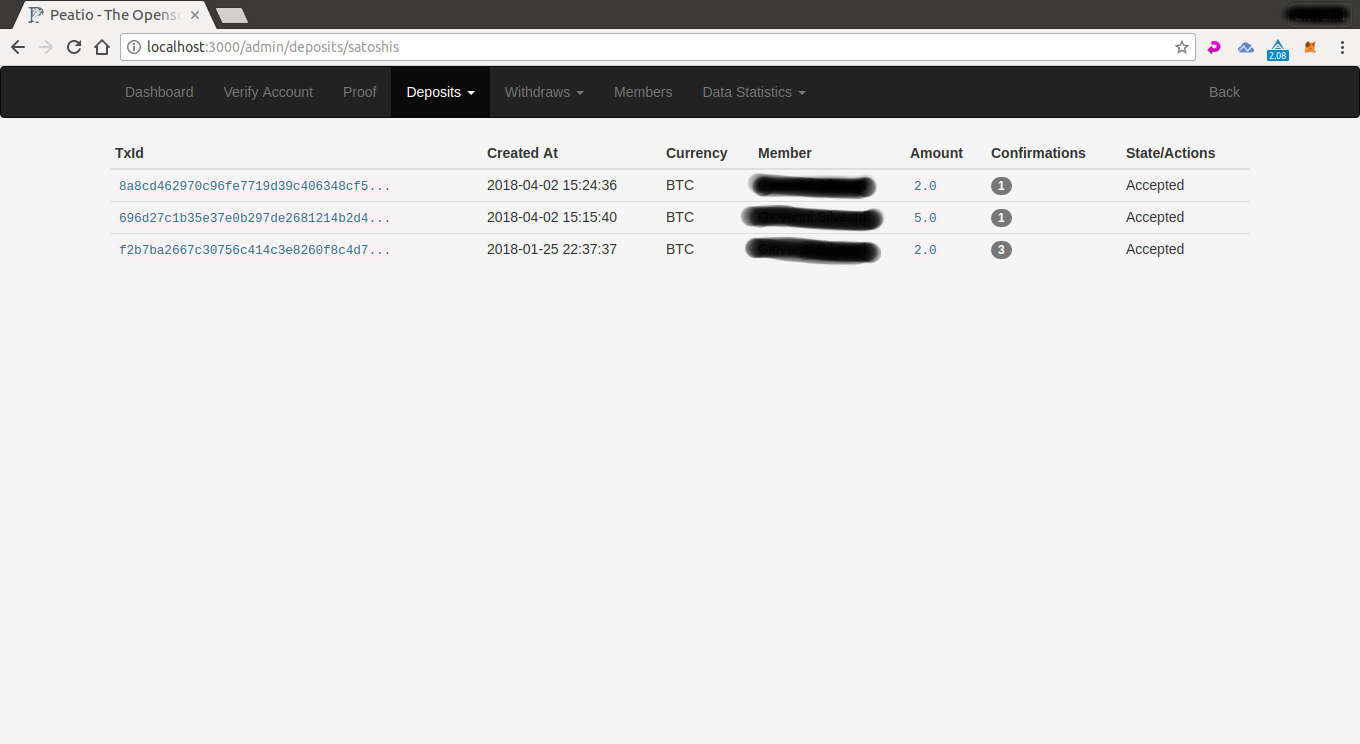
\includegraphics[width=\textwidth*2/3,height=\textheight,keepaspectratio]{RE_adminDepositsC}
	\captionof{figure}{Ripa Exchange Admin console deposit screen}
	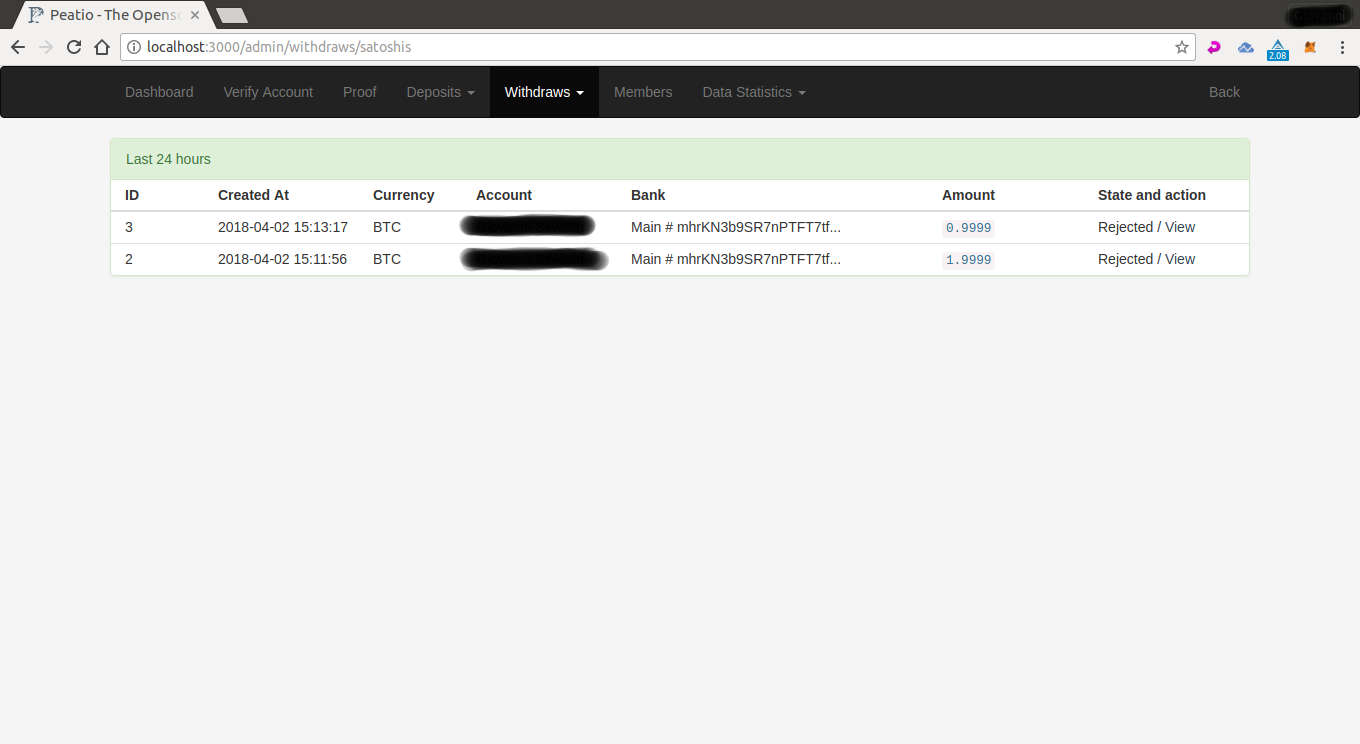
\includegraphics[width=\textwidth*2/3,height=\textheight,keepaspectratio]{RE_adminWithdrawsC}
	\captionof{figure}{Ripa Exchange Admin console whitdraw screen}
	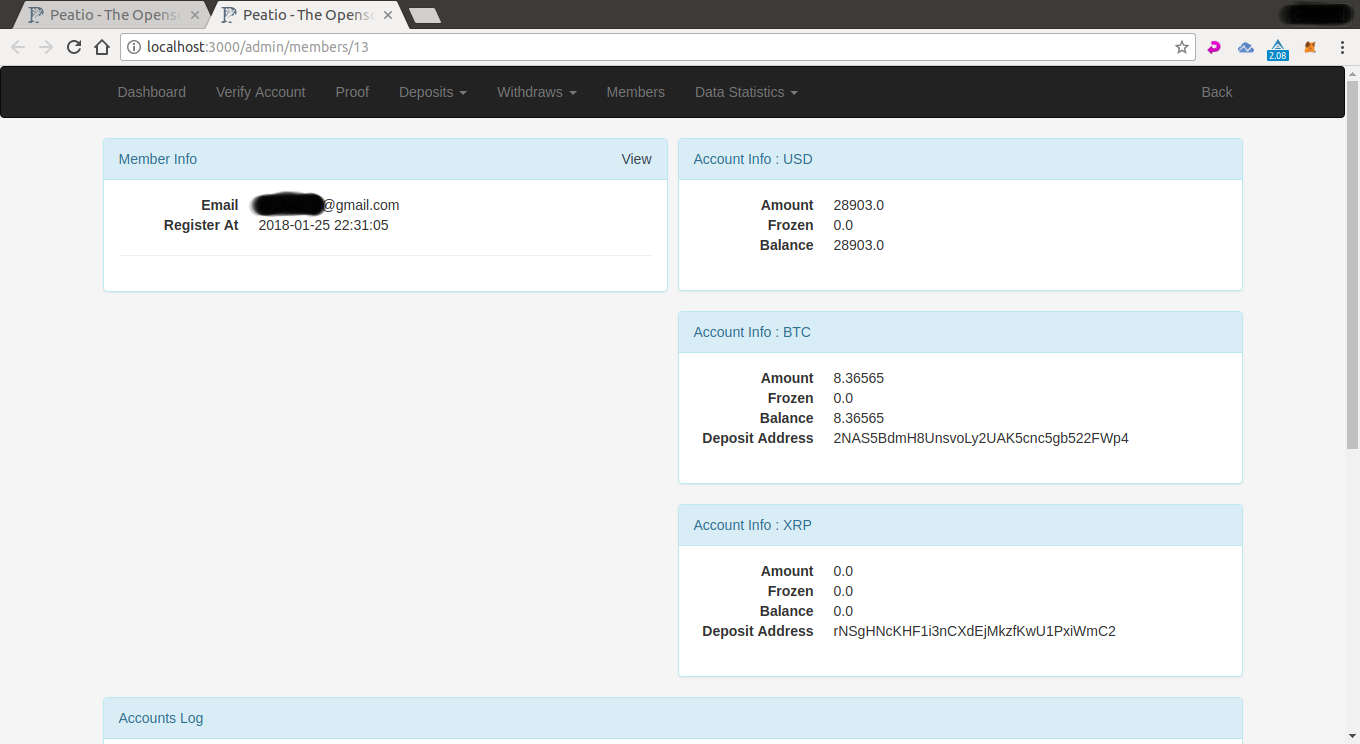
\includegraphics[width=\textwidth*2/3,height=\textheight,keepaspectratio]{RE_adminUserInfo1C}
	\captionof{figure}{Ripa Exchange Admin user info screen}
	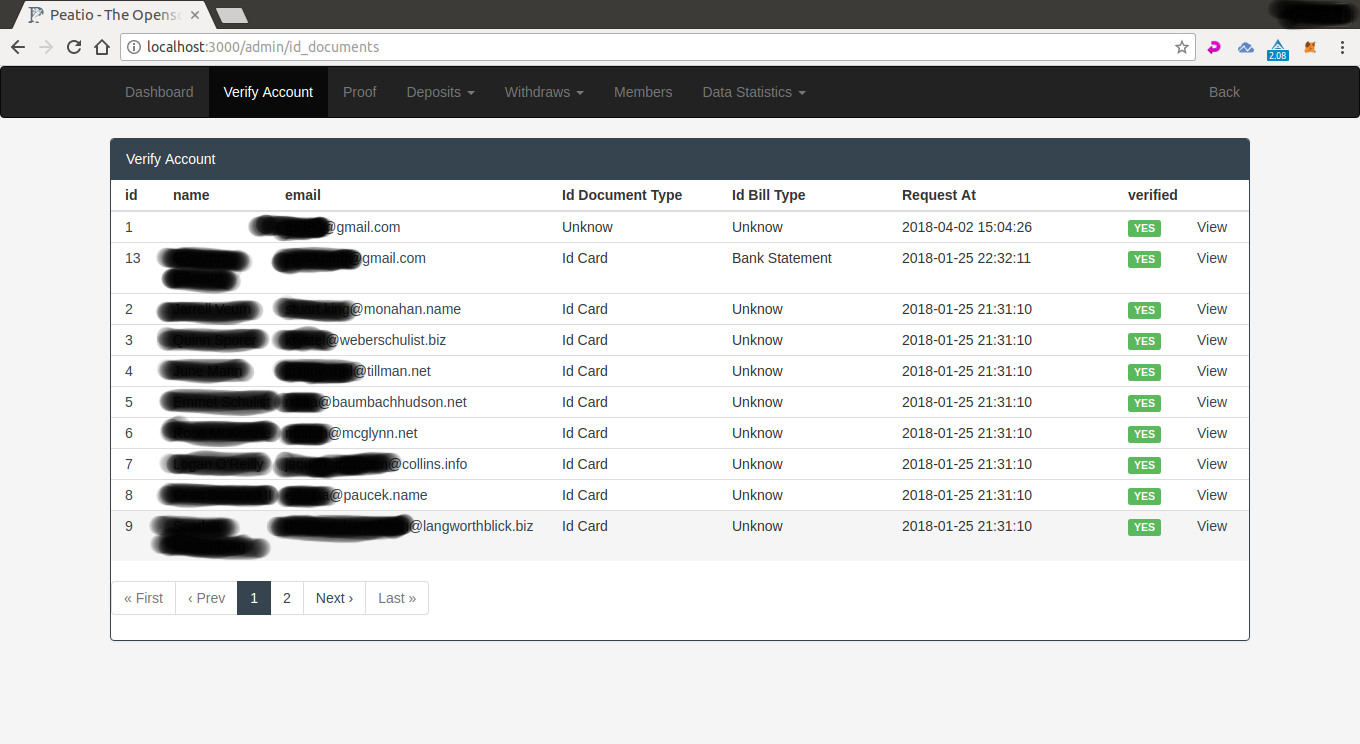
\includegraphics[width=\textwidth*2/3,height=\textheight,keepaspectratio]{RE_adminVerifyAccountC}
	\captionof{figure}{Ripa Exchange Admin verify account screen}
\end{center}

\section{Features at Launch}
At the first working Ripa Exchange instance opening the following features will be functioning:
\begin{itemize}
	\item \textsc{CRYPTO $\Leftrightarrow$ CRYPTO}:
	\item \textsc{OAuth}: Facebook, Google, Twitter
	\item \textsc{FIDO}: login with FIDO Alliance standards
	\item \textsc{Protocols}: POW, DPOS, Masternode, tether, ERC20
	\item \textsc{Currencies}: BTC, ETH, DOGE, BCH, TUSD, ARK, LISK, SHIFT, RISE, KAPU, OXY, RIPA, promising ERC20 tokens
	\item \textsc{Main Markets}: BTC, ETH, ARK
	\item \textsc{Orders Type}: market, limit
\end{itemize}

\subsection{Future Features}
Future instances of Ripa Exchange implementations will have the following features:
\begin{itemize}
	\item \textsc{E-Wallets}: OKPay, NETELLER, MoneyPolo, others...
	\item \textsc{Advanced Trading Features}: margin trading, stop loss and take profit, 
	\item \textsc{FIAT $\Leftrightarrow$ CRYPTO}
	\item \textsc{Other tools}: VISA/MasterCard, merchants tools, P2P Lending 
\end{itemize}


\section{Towards a Decentralized Exchange...}
Ripa Exchange is a centralized exchange which will be converted into an hybrid-decentralized exchange to create a network of exchanges
that share the same liquidity between each of them so you can offer liquidity from day 1 of your exchanges operations.\\

To offer the PROs of a centralized exchange like platinum customer support and FIAT exchange, with all the PROs of a 
decentralized exchange like liquidity, without the CONs of both of them, 
we need to perform an intermediate step where Ripa Exchange will be converted into an hybrid-decentralized exchange 
and during phase 3 of our project (WP4-6) we will make all the functional and technical analysis required 
to make the next step on solid ground and offer to the RipaEx community an open source, secure and efficient exchange.
